\chapter{Contribution}\label{sec:contribution}

Most important chapter of the thesis. Describes what the author contributes as research. Discusses intuition, motivation, describes and reasons about necessity of proposed elements. Defines theses based on reasonable assumptions. Discusses relevant aspects of contribution. Approximately 30 to 40 pages. Can be split into multiple chapters.
\\\\

\section{Baumlayout}

\subsection{Linear vs. Radial}\label{sec:radial}
Aufgrund des begrenzten Platzes, der auf mobilen Geräten typischerweise zur Verfügung steht, ist zu entscheiden, wie Baumstrukturen möglichst platzsparend anzuordnen sind, ohne Übersichtlichkeit einzubüßen. Betrachtet werden dazu speziell die allgemein übliche Darstellung (linear) gegenüber einer kreisförmigen (radialen) Anordnung.\\
\begin{figure}
	\centering
	\begin{minipage}{.5\textwidth}
		\centering
		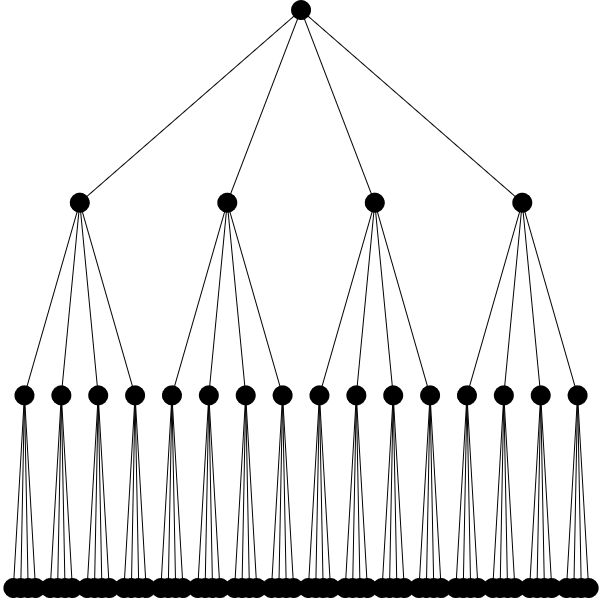
\includegraphics[width=.9\linewidth]{../screenshots/lineargraphexample.PNG}
		\caption{Lineare Baumdarstellung}
		\label{abb:linearbaum}
	\end{minipage}%
	\begin{minipage}{.5\textwidth}
		\centering
		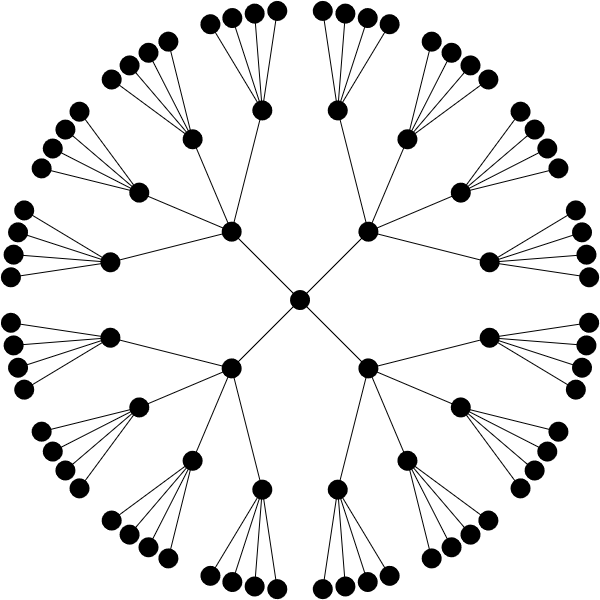
\includegraphics[width=.9\linewidth]{../screenshots/radialgraphexample.PNG}
		\caption{Radiale Baumdarstellung}
		\label{abb:radialbaum}
	\end{minipage}
\end{figure}
Die Abbildungen \ref{abb:linearbaum} und \ref{abb:radialbaum} zeigen einen Vergleich zwischen einem Baum in linearer (Abb. \ref{abb:linearbaum}) und in radialer Anordnung (Abb. \ref{abb:radialbaum}). In beiden Fällen ist derselbe Baum der Höhe 4 auf gleicher Fläche abgebildet. Er besteht aus 105 Knoten, wobei alle inneren Knoten jeweils vier Nachfolger haben. Der Wurzelknoten befindet sich beim linearen Layout am oberen Rand. Die übrigen Knoten sind in drei horizontalen Linien darunter angeordnet, wobei die Kinder der Wurzel auf der obersten Linie liegen, deren Kinder auf der mittleren und deren Kinder auf der untersten Linie. Beim radialen Layout ist die Wurzel in der Mitte abgebildet und alle anderen Knoten in drei konzentrischen Kreisen darum herum. Knoten der Tiefe 1 liegen auf dem innersten Kreis, der Tiefe 2 auf dem mittleren Kreis und die Blätter auf dem äußeren Kreis. Den Mittelpunkt der Kreise bildet die Wurzel. Man sieht deutlich, dass im Fall der vertikalen Anordnung (Abb. \ref{abb:linearbaum}) nicht ausreichend Platz für alle Blätter zur Verfügung steht, wodurch es zu Überschneidungen kommt. In der radialen Anordnung (Abb. \ref{abb:radialbaum}) können hingegen alle Knoten überschneidungsfrei dargestellt werden.

Um den Grund dafür zu veranschaulichen vergleicht man den Platz, der bei den beiden Herangehensweisen auf einer einzelnen Stufe des Baumes zur Verfügung steht. Unter der Annahme, dass für die gesamte Darstellung ein Quadrat mit Seitenlänge $a$ zur Verfügung steht und alle Knoten einen Durchmesser von 1 haben ergibt sich für den Platz $l_{linear}$ bzw. $l_{radial}$, der auf einer Stufe des Baumes verfügbar ist 
\begin{align*}
&l_{linear} = a\\
&l_{radial} = 2 \cdot \pi \cdot r\mspace{40mu} mit\quad 0\leq r \leq \frac{a}{2} .
\end{align*}
Dabei bezeichnet $r$ den Abstand einer Stufe zum Wurzelknoten. Setzt man $l_{radial}$ und $l_{linear}$ gleich und stellt nach $r$ um, so ergibt sich
\begin{align*}
&l_{linear} = l_{radial}\\
\Rightarrow \mspace{40mu} &a = 2 \cdot \pi \cdot r\\
\Rightarrow \mspace{40mu} &\frac{a}{2 \cdot \pi} = r\\
\Rightarrow \mspace{40mu} &r \approx \frac{a}{6}.
\end{align*}
Da $l_{linear}$ konstant ist kann man daraus ableiten
\begin{align*}
l_{radial} > l_{linear} \mspace{40mu} \Leftrightarrow  \mspace{40mu} r > \frac{a}{6}.
\end{align*}
Das bedeutet, dass ab einem Abstand zur Wurzel von mehr als $\frac{a}{6}$ im radialen Layout mehr Platz für jede Stufe verfügbar ist. Außerdem gilt: Je größer der Abstand $r$, desto mehr Platzersparnis. Das ist vor allem deshalb von Interesse, weil Bäume in der Regel die Eigenschaft haben, dass mit wachsender Baumtiefe auch die Anzahl der Knoten in der jeweiligen Tiefe wächst und diese tiefer liegenden Knoten in der kreisförmigen Darstellung weiter von der Wurzel entfernt sind. Das radiale Layout bietet somit genau dann mehr Platz, wenn üblicherweise mehr Platz benötigt wird.
Aufgrund dieser Erkenntnis und der Tatsache, dass beide Darstellungsformen gute Übersichtlichkeit aufweisen, fiel die Wahl letztendlich auf das radiale Layout.

\subsection{Polarkoordinaten}\label{sec:polarkoordinaten}
D3 bietet zur Berechnung einer sinnvollen Knotenanordnung von Bäumen die Funktion $d3.tree$ an, welche unter Verwendung des Reingold-Tilford Algorithmus \todo{quelle} allen Knoten einer $hierarchy$ x- und y-Koordinaten jeweils im Bereich von 0 bis 1 zuordnet. Es liegt dann in der Hand des Programmierers, diese sinnvoll zu interpretieren. Um die Knoten, wie in Abbildung \ref{abb:radialbaum} gezeigt in konzentrischen Kreisen anzuordnen, eignen sich Polarkoordinaten ausgezeichnet. Einem Vorschlag aus der Dokumentation von D3 folgend \todo{quelle} wird die y-Koordinate als Radius $\rho$, die x-Koordinate als Polarwinkel $\varphi$ in Radiant interpretiert. \todo{bild}
\begin{align*}
&\rho = y\\
&\varphi = 2 \cdot \pi \cdot x
\end{align*}
Zur Darstellung auf dem Bildschirm müssen $\rho$ und $\varphi$ anschließend in kartesische Koordinaten $x_{screen}$ und $y_{screen}$ umgerechnet werden. Die allgemeinen Umrechnungsformeln ergeben sich als
\begin{align*}
&x_{screen} = \rho \cdot \cos (\varphi)\\
&y_{screen} = \rho \cdot \sin (\varphi).
\end{align*}
Bei dieser Umrechnung wird allerdings noch nicht berücksichtigt, dass die gegebenen Polarkoordinaten auf generischen Koordinaten im Bereich $[0,1]$ basieren. Zur korrekten Positionierung müssen noch eine Skalierung auf die verfügbare Breite (width) $w$ und Höhe (height) $h$, sowie eine Verschiebung in die Mitte der Anzeige vorgenommen werden. Es entstehen die endgültigen Formeln:
\begin{align}
&x_{screen} = \rho \cdot \cos (\varphi) \cdot w + \frac{w}{2} \label{eq:polkarthx}\\
&y_{screen} = \rho \cdot \sin (\varphi) \cdot h + \frac{h}{2}.\label{eq:polkarthy}
\end{align}

\section{Reduzieren der angezeigten Knoten}\label{sec:reduzieren}
Nachdem mit dem radialen Layout (Kapitel \ref{sec:radial}) eine erste Maßnahme zum Einsparen von Platz ergriffen wurde, stellt sich als nächstes die Frage, wie die Übersichtlichkeit weiter verbessert werden kann. Da Knoten auf dem Bildschirm Informationen in Form von Text beinhalten sollen, ist es abzusehen, dass jeder einzelne Knoten mehr Platz einnehmen wird, als z.B. in Abbildung \ref{abb:radialbaum} gezeigt ist. Es bietet sich an, immer nur aktuell relevante Knoten ein- und irrelevante auszublenden. Das erfordert je nach Eingabe dynamische Änderungen an der Anzeige der Baumstruktur (Kapitel \ref{sec:dynamische_aktual}). Zunächst muss jedoch entschieden werden, welche Knoten aktuell relevant oder irrelevant sind. 

Dazu betrachten wir noch einmal den simplen Entscheidungsbaum in Abbildung \ref{abb:entsch_baum_bsp}. Die beiden Stellen, an denen Entscheidungen getroffen werden müssen, sind dort mit $A$ und $B$ markiert. In Situation $A$ gilt es zu entscheiden, ob es regnet oder nicht. Um diese Entscheidung treffen zu können, ist nicht relevant, ob es zu einem späteren Zeitpunkt regnen wird oder nicht und welche Ergebnisse sich daraus ableiten lassen. Bei $B$ wiederum sind vorherige Entscheidungsmöglichkeiten nicht von Interesse, ebenso wie die Folgen davon, ob es regnen wird oder nicht. Man kann sagen, dass bei jeder Verzweigung nur die zur Verfügung stehenden Alternativen relevant sind und angezeigt werden müssen. Da es jedoch nicht nur darum geht, so viel Platz wie möglich zu sparen, sondern auch darum, eine übersichtliche und intuitiv verständliche Darstellung zu finden ist es hilfreich, außerdem noch den Knoten, von dem die Verzweigung ausgeht zu zeigen. Bei $A$ also den Knoten \glqq Regenschirm nötig\grqq , bei $B$ \glqq Es regnet nicht\grqq . Auf diese Art ist es leichter die Orientierung zu behalten, selbst wenn ein Großteil des Baumes nicht sichtbar ist.

Das Grundlegende Konzept, bestehend aus dem radialen Layout und dem Weglassen irrelevanter Knoten, kann nun unter Verwendung von D3 umgesetzt werden.

\section{Baumdarstellung mit D3}

Um mit D3 auf den Bildschirm zu zeichnen gibt es verschiedene Möglichkeiten. In der Regel werden die HTML-Elemente $canvas$ oder $svg$ als Zeichenfläche verwendet. Beide haben Vor- und Nachteile, die vor einer Entscheidung abzuwägen sind.

\subsection{Vergleich zwischen Canvas und SVG}\label{sec:cvs}
Der größte Unterschied zwischen $canvas$ und $svg$ Elementen besteht darin, dass ein $svg$ jedes Objekt, dass es anzeigen soll einzeln als HTML-Element hinterlegt während ein $canvas$ nur das insgesamt entstehende Bild speichert. Für den Browser bedeutet das, dass bei einem $canvas$ nur die Darstellung eines  einzelnen Bildes zu berechnen ist, während bei einem $svg$ alle dargestellten Objekte getrennt behandelt werden. Das führt dazu, dass mit wachsender Zahl anzuzeigender Elemente die Berechnungsdauer des $svg$ stärker ansteigt, als die des $canvas$. Das einzelne Speichern der Anzeigebausteine bringt aber auch Vorteile mit sich. Es ist einfach ein einzelnes Objekt auf dem Bildschirm zu verändern, indem man dessen $svg$-Attribute anpasst, weil der Browser sich dann selbst um die Aktualisierung der Anzeige kümmert. D3 bietet mit seinen $transitions$ eine simple Möglichkeit beliebige Animationen auf einem $svg$ Element durchzuführen, was auf einem $canvas$ umständlicher mit D3 $interpolators$ und einer Funktion zu lösen ist, die für jedes Einzelbild der Animation das Bild neu zeichnet. Allgemein scheint die Nutzung eines $svg$-Elements zur Darstellung von Daten mit D3 die am häufigsten gewählte Herangehensweise, was zu einer großen Menge Beispiele führt, die zur Inspiration genutzt werden können. Auch in diesem Fall fällt die Wahl darauf D3 in Verbindung mit $svg$ einzusetzen. Diese Entscheidung wird vor allem durch die in Kapitel \ref{sec:reduzieren} beschriebene Reduzierung der angezeigten Knoten untermauert, denn der große Vorteil schnellerer Berechnung auf $canvas$-Elementen fällt damit kaum noch ins Gewicht.

\subsection{Datenstruktur}
Zur Speicherung der Baumdaten werden die Knoten in eine D3 $hierarchy$ Umgewandelt. Es ist zu beachten, dass eine $hierarchy$ nur durch ein einzelnes Objekt repräsentiert wird, welches die Wurzel ($root$) des Baumes darstellt. Um eine Liste aller Knoten zu erhalten kann $root.descendants$ aufgerufen werden. Jeder einzelne Knoten ist dabei ein Javascript-Objekt, das die in Kapitel \ref{sec:inputdaten} beschriebenen Daten enthält. Wendet man die Funktion $d3.tree$ (Kapitel \ref{sec:hierarchies}) auf die $hierarchy$ an, so kommen zusätzlich noch x- und y-Koordinaten dazu. Unter Einsatz dieser Daten kann der Baum in einem $svg$-Element dargestellt werden.

\subsection{Erzeugung eines SVG}\label{sec:svgcreate}
Zu Beginn wird dem HTML-Dokument mit $d3.select$ und $selection.append$ ein $svg$-Element angehängt. Die Rückgabe von $append$ - eine $selection$, die nur das $svg$ enthält - wird in einer Variable zwischengespeichert.

\begin{figure}
	\centering
	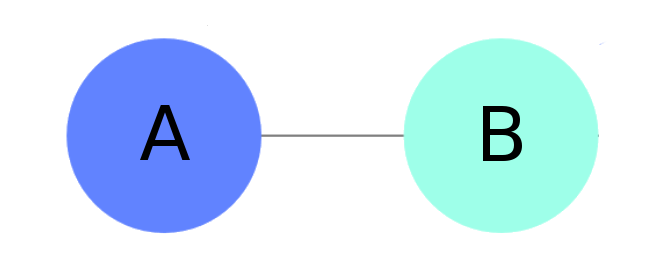
\includegraphics[width=\linewidth]{../screenshots/knotendesign.PNG}
	\caption{Konzept für Knoten- und Kantendarstellung}
	\label{abb:design}
\end{figure} 
Abbildung \ref{abb:design} zeigt das gewünschte Aussehen für Knoten und Kanten. Zu sehen sind zwei Knoten als Kreise mit Beschriftung A und B. Die Kante zwischen den Beiden Knoten ist dargestellt als Linie, die beide Kreise miteinander verbindet. Die Unterschiedlichen Farben der Knoten zeigen an, dass sie verschiedene Knotentypen haben. Im medizinischen Kontext könnte es sich zum Beispiel um ein Symptom A und eine Diagnose B handeln. Es ergibt Sinn, für Knoten und Kanten getrennte Gruppen zu erstellen. Dazu werden unter der Verwendung der zuvor gespeicherten $selection$ zwei $g$-Elemente hinzugefügt, die im Folgenden als Knoten- und Kantengruppe bezeichnet werden.

\subsection{Präparieren der Knotendaten für die Darstellung}\label{sec:prep}
Bevor die Knoten auf den Bildschirm gebracht werden können, müssen zunächst deren Koordinaten bestimmt werden. Außerdem soll darauf geachtet werden, dass wie in Kapitel \ref{sec:reduzieren} erörtert nur der aktuelle Verzweigungsknoten und dessen Kinder angezeigt werden. Die zur Koordinatenberechnung verwendete Funktion $d3.tree$ erhält als Übergabe einen Startknoten und läuft bei der Berechnung von dort den gesamten nachfolgenden Baum ab, wobei jedem Knoten x- und y-Koordinaten gegeben werden. Dazu verwendet sie immer die Liste $children$, die in jedem Knoten enthalten ist und dessen Kinder aufzählt. Erreicht die Funktion einen Knoten, der kein $children$-Objekt enthält, dann wird dieser als Blatt betrachtet. Da nur ein Knoten und dessen Nachfolger in die Berechnung einbezogen werden sollen, muss $d3.tree$ die Nachfolger dieses Knotens als Blätter betrachten. Das wird erreicht, indem die $children$-Objekte der Kinder entfernt und in einem $childrenBackup$ benannten Objekt zwischengespeichert werden. Hat $d3.tree$ anschließend allen anzuzeigenden Knoten ihre Koordinaten zugewiesen, werden diese noch mit dem in Kapitel \ref{sec:polarkoordinaten} beschriebenen Verfahren umgerechnet, um eine Kreisförmige Anordnung zu erzeugen.

Ein weiterer Voreilt dieses Verfahrens liegt darin, dass zum Erhalten einer Liste der anzuzeigenden Knoten $currentRoot.descendants$ aufgerufen werden kann, weil auch diese Funktion die $children$ Objekte zum ablaufen des Baumes verwendet. Das Objekt $currentRoot$ bezeichnet dabei den aktuellen Verzweigungsknoten.

\subsection{Erzeugen der Knotendarstellung}\label{sec:knoten}

Wie auf Abbildung \ref{abb:design} zu sehen ist, soll die Knotenvisualisierung aus einem Kreis mit einer Aufschrift bestehen. Für jeden Knoten muss das $svg$ also ein $circle$ und ein $text$-Element enthalten. Um leichter beide zusammen ein- und ausblenden sowie verschieben zu können, sollen diese jeweils Gruppiert werden. Mit $selectAll$ wählt man zuerst alle $g$-Elemente in der Knotengruppe aus und Verknüpft diese unter Einsatz von $selection.data$ mit den gewünschten Knotendaten, welche nach dem gerade beschriebenen Präparieren der Daten mit $currentRoot.descendants$ zu erhalten sind. Die daraus entstehende $enter\ selection$ verwendet man dann um für alle neu hinzugekommenen Knoten $g$-Elemente einzufügen, die einen $circle$ mit zentriertem $text$ enthalten. Der Radius des Kreises ist abhängig von der Bildschirmgröße und der Text wird den Knotendaten entnommen. Mit dem $transform$-Attribut der $g$-Elemente werden die Gruppen an die zuvor berechneten Koordinaten geschoben.

Wegen der begrenzten Bildschirmgröße von mobilen Geräten soll die Knotenaufschrift zur besseren Lesbarkeit so groß wie möglich sein, ohne den Kreis zu überschreiten, in dem sie zentriert ist.

\subsubsection*{Berechnen der Schriftgröße}
\todo{aufteilung auf zwei zeilen implementieren}
\todo{bild von Knoten mit langem text}
Angaben von Schriftgrößen beziehen sich auf die Höhe der Buchstaben \todo{quelle}. Das bedeutet nicht notwendigerweise, dass eine Schriftgröße von 10px zu Buchstaben führt, die exakt Zehn Pixel hoch sind, sondern dass die Höhe der Schriftzeichen proportional zur angegebenen Schriftgröße ist. Das bedeutet auch, dass die Breite eines Buchstabens dazu proportional ist, da er beim Vergrößern nicht verzerrt werden soll, wodurch das Verhältnis von Höhe zu Breite immer gleich bleibt. Diese Tatsache lässt sich auf ganze Texte übertragen...

\subsection{Erzeugen der Kantendarstellung}\label{sec:kanten}
Die Darstellung der Kanten verläuft analog zur Knotendarstellung in Kapitel \ref{sec:knoten}, allerdings werden anstelle von $g$-Elementen mit $circle$ und $text$ jetzt $path$-Elemente verwendet. Zur Erzeugung der $enter\ selection$ wird als Daten die Rückgabe der $hierarchy$-Funktion $node.links$ verwendet, welche eine Liste aller Kanten, die von einem Knoten ausgehen, zurückgibt. Aus den Einträgen dieser Liste lassen sich mit $d3.line$ die Zeichenanweisungen für das $d$-Attribut der $path$-Elemente berechnen.

\section{Navigation im Baum}
Durch das Ausblenden vieler der Knoten muss nun eine Möglichkeit geschaffen werden, von einer Entscheidung zur nächsten zu navigieren, wobei immer wieder irrelevante Knoten aus- und relevant gewordene eingeblendet werden. Das wird möglich gemacht, indem die Baumanzeige auf Berührung hin dynamisch aktualisiert wird. Es gilt dabei, dass der Knoten, von dem die aktuelle Verzweigung ausgeht, in der Mitte des Bildschirms zu sehen ist und die nachfolgenden Entscheidungsmöglichkeiten im Kreis darum herum angeordnet werden.
\begin{figure}
	\centering
	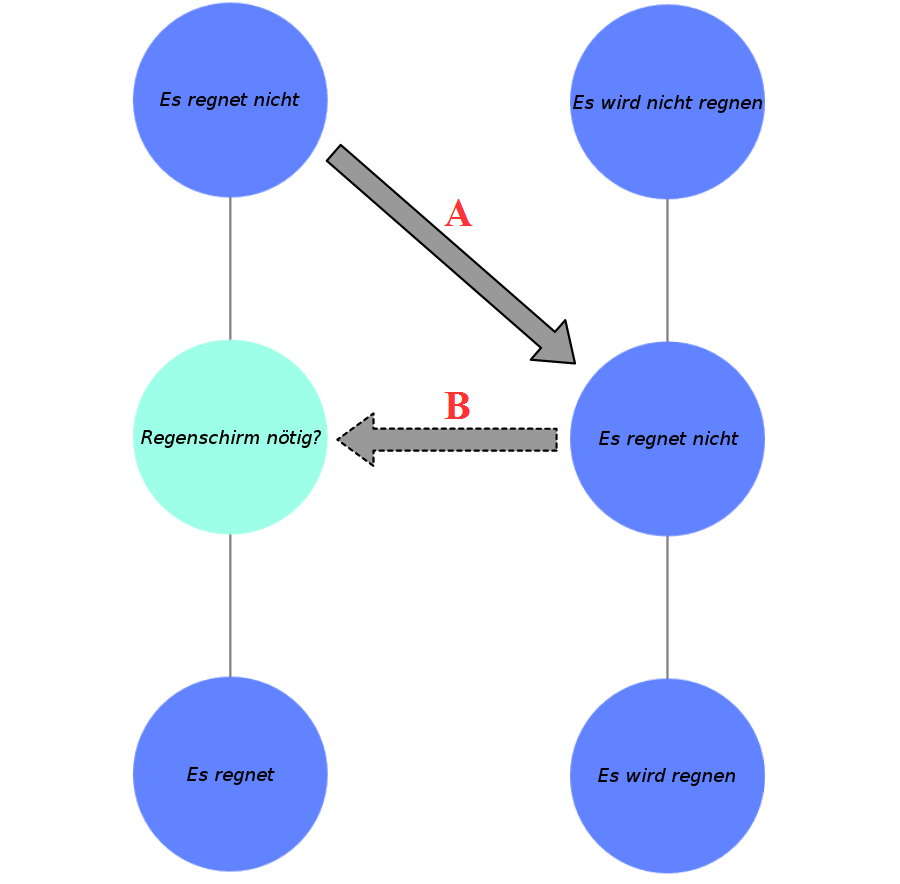
\includegraphics[width=.7\linewidth]{../screenshots/baumnavigation.PNG}
	\caption{Beispiel zur Baumnavigation}
	\label{abb:baumnavigation}
\end{figure}
Abbildung \ref{abb:baumnavigation} zeigt die Reaktion des Baumes auf verschiedene Nutzereingaben. Auf der linken Seite ist der Ausgangszustand zu sehen und rechts der Nachfolgezustand. Links ist der mittlere Knoten mit \glqq Regenschirm nötig?\grqq\ beschriftet und dessen Nachfolger mit \glqq Es regnet nicht\grqq\ sowie \glqq es regnet\grqq. Rechts sieht man \glqq Es regnet nicht\grqq\ in der Mitte, \glqq Es wird nicht regnen\grqq\ und \glqq Es wird regnen\grqq\ als Folgeknoten. Die mit $A$ und $B$ beschrifteten Pfeile symbolisieren Reaktionen auf Eingaben, die im Folgenden genauer beschrieben werden. 

Durch Antippen eines der äußeren Knoten wird dieser in die Mitte verschoben und es zeigen sich dessen Nachfolger. Tippt man zum Beispiel in Abbildung \ref{abb:baumnavigation} links \glqq Es regnet nicht\grqq\ an, dann wird dieser, wie Pfeil $A$ zeigt, zum mittleren Knoten, die anderen verschwinden und es erscheinen die neuen Nachfolgeknoten. Möchte man einen Schritt zurück machen, kann der Mittelknoten berührt werden und man wird wieder zur links gezeigten Situation geleitet (illustriert durch Pfeil $B$). Es soll dadurch das Gefühl entstehen, dass man sich durch die Baumstruktur bewegt, wobei besonders die gewählten Animationen (Kapitel \ref{sec:animation}) von großer Wichtigkeit sind. Zuerst ist aber zu klären, wie die interne Datenstruktur verwendet werden kann, um dynamische Aktualisierungen zu ermöglichen.
  
\subsection{Dynamische Aktualisierung}\label{sec:dynamische_aktual}
Mit dem Präparieren der Daten in Kapitel \ref{sec:prep} ist bereits der Grundstein für das Aktualisieren der Anzeige auf Nutzereingaben hin gelegt worden. Wird einer der Entscheidungsknoten berührt, so soll dieser zum neuen mittleren Knoten werden und dessen Nachfolger darum herum erscheinen (Abbildung \ref{abb:baumnavigation}). Dazu wird als erstes das $children$-Objekt des ausgewählten Knotens, welches beim Präparieren der vorherigen Daten in das Objekt $childrenBackup$ verschoben wurde, wiederhergestellt. Anschließend werden mit dem angetippten Knoten als Verzweigungsknoten die Schritte vom Präparieren der Daten bis zur Anzeige erneut durchgeführt (Kapitel \ref{sec:prep} bis \ref{sec:kanten}). Der Unterschied besteht diesmal aber darin, dass nicht nur die $enter\ selections$ beim Verknüpfen der Daten betrachtet werden, sondern auch die $update-$ und $exit\ selections$. Die $update\ selection$ enthält dann den neuen Mittelknoten, weil er bereits vorher auf dem Bildschirm war. Dieser muss nur an seine neue Position in der Mitte der Anzeige verschoben werden, indem das $transform$-Attribut seines $g$-Elements angepasst wird. In der $exit\ selection$ befinden sich der vorherige Verzweigungsknoten und dessen Kinder, die nicht ausgewählt wurden. Sie werden mit der Funktion $selection.remove$ vom Bildschirm entfernt. \todo{verweise auf abbildung zur veranschaulichung}


\section{Eingabemenü}\label{sec:eingabemenu}
\begin{figure}
	\centering
	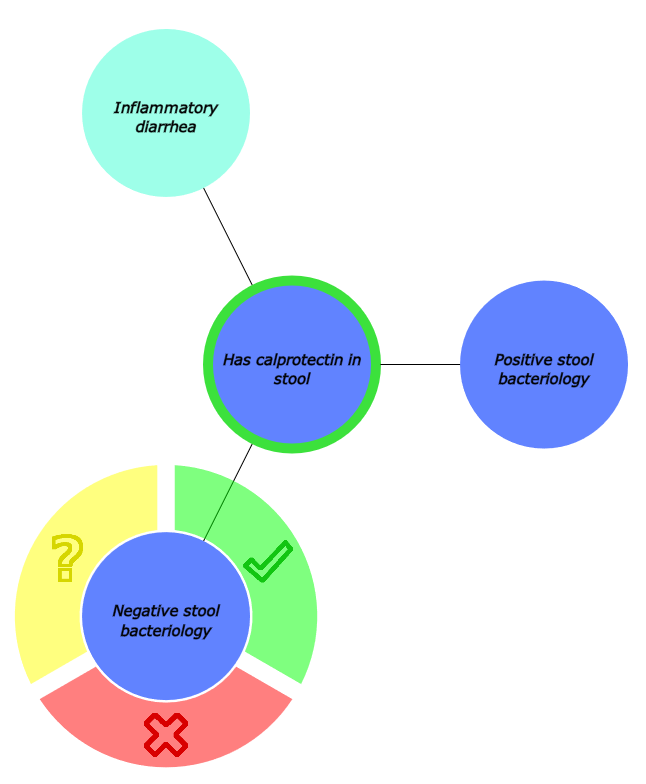
\includegraphics[width=.6\linewidth]{../screenshots/eingabemenu.PNG}
	\caption{Eingabemenü zum Eintragen von Untersuchungsergebnissen}
	\label{abb:eingabemenu}
\end{figure} 
\section{Einsatz von Animationen}\label{sec:animation}
Häufig kommen bei der hier beschriebenen interaktiven Visualisierung Animationen zum Einsatz und spielen dabei für diverse Aspekte eine zentrale Rolle. \todo{verweise auf material design guidelines}

\subsection{Interaktivität}
Für eine interaktive Anwendung ist es wichtig, dass Nutzer immer das Gefühl haben, dass sie das Geschehen auf dem Bildschirm kontrollieren. Das ist nicht gewährleistet, wenn sich Elemente auf Eingaben hin unvorhersehbar oder nicht nachvollziehbar verhalten. Durch kontinuierliche Bewegungen, wie in Abbildung \ref{abb:animation}, anstelle von plötzlichen Sprüngen kann immer nachvollzogen werden, wie die Visualisierung sich verändert, womit eine interaktivere Umgebung geschaffen wird.

\subsection{Verbesserung von Orientierung und Übersichtlichkeit}
Kapitel \ref{sec:reduzieren} beschreibt, wie zum Einsparen von Platz Knoten weggelassen werden können. Ein daraus folgender Nachteil besteht im Orientierungsverlust. Obwohl die Menge an Informationen auf dem Bildschirm sinkt, was die Übersichtlichkeit verbessert, wird es schwerer zu wissen, wo man sich im Baum gerade befindet. Durch passende Animationen beim in Kapitel \ref{sec:dynamische_aktual} beschriebenen dynamischen Aktualisieren des Baumes kann dem Abhilfe geschaffen werden. Es soll dabei durch die Bewegungen auf dem Bildschirm deutlich werden, welche Veränderung eine Eingabe bewirkt.
\begin{figure}
	\centering
	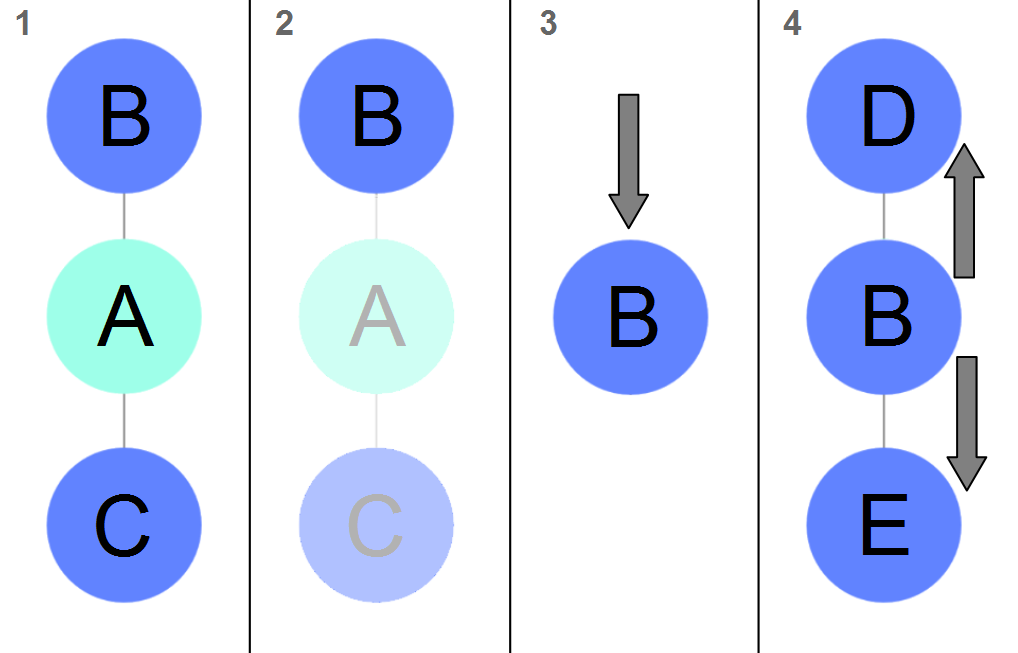
\includegraphics[width=.9\linewidth]{../screenshots/animation.png}
	\caption{Animation beim Berühren eines Knotens}
	\label{abb:animation}
\end{figure}
Die gewählte Animation beim Navigieren von einem Knoten zum nächsten ist in Abbildung \ref{abb:animation} zu sehen. Von links nach rechts mit 1 bis 4 nummeriert werden die vier wichtigen Zeitpunkte im Bewegungsablauf gezeigt. Situation 1 zeigt den Ausgangszustand: Ein Knoten $A$ mit dessen Nachfolgerknoten $B$ und $C$. Die anderen drei Stadien zeigen was geschieht, wenn man $B$ antippt. Zunächst werden bei 2 die Knoten $A$ und $C$ durchsichtiger, bis sie nicht mehr zu sehen sind. Anschließend bewegt sich $B$ in die Mitte der Anzeige (zu sehen bei 3) und zuletzt bewegen sich zu Zeitpunkt 4 von $B$ aus die Knoten $D$ und $E$ nach außen.

Das Ausblenden von $A$ und $C$ verdeutlicht, dass beide nicht mehr relevant sind, geschieht aber zur Vermeidung von Verwirrung nicht von einem Moment auf den anderen. Die Bewegung von $B$ in die Mitte lässt leicht nachverfolgen, dass $B$ zum neuen Verzweigungspunkt wird. Wichtig ist dabei, dass $B$ zu keinem Zeitpunkt vom Bildschirm verschwindet oder umherspringt, wodurch klar ist, dass es sich noch immer um denselben Knoten handelt. Zuletzt verdeutlicht die von $B$ ausgehende Bewegung von $D$ und $E$ nach außen, dass diese die Nachfolger von $B$ sind. Der allgemeine Schwerpunkt liegt darauf, es durch kontinuierliche Bewegungen leichter zu machen, dem Geschehen zu folgen, was zu einem intuitiven Verständnis der Vorgänge auf dem Bildschirm führt.



























































